\documentclass[11pt]{article}
\usepackage[utf8]{inputenc}
\usepackage[T1]{fontenc}
\usepackage[margin=1in]{geometry}
\usepackage{array}
\usepackage{booktabs}
\usepackage{graphicx}
\usepackage{hyperref}
\usepackage{longtable}
\usepackage{float}

\title{MedGuard-CXR: A Safety-Aware Chest X-ray Pneumonia Detection and Evidence Prototype\\
\large Current NIH Classifier Training Results and Continuation Plan for Calibration, RSNA Grounding, and Safe VQA}
\author{Anıl Keskin}
\date{May 10, 2026}

\begin{document}
\maketitle

\begin{center}
\textbf{Safety notice:} MedGuard-CXR is a research and engineering prototype only. It is not a clinical diagnostic tool and must not be used for patient care.
\end{center}

\section{Introduction}

MedGuard-CXR is a safety-aware chest X-ray engineering prototype. The project combines a DenseNet121 image classifier, calibration and abstention logic, pneumonia-specific RSNA grounding checks, and a rule-based VQA/API/demo layer that keeps research-only disclaimers visible.

The purpose of this report is to publish the current real NIH classifier results and to preserve the continuation plan for calibration, RSNA grounding, and safe VQA work. The system is not a clinical diagnostic tool, has not been prospectively evaluated, and must not be used for patient care.

The current repository status is explicitly \textbf{REAL COMPLETED}: NIH classifier training, NIH evaluation, calibration, and RSNA Pneumonia grounding artifacts exist. By contrast, the \textbf{IDEALIZED FUTURE / NOT YET RUN} path includes broader VLM/QLoRA training, free-text VLM validation, clinical validation, and any other aspirational model-training milestones that are not present in the current repository artifacts. Phase 4A VQA/API/Gradio remains rule-based and smoke-tested. Phase 4B VLM/QLoRA is deferred and not trained.

\subsection{Research Questions}

\textbf{RQ1: does per-class post-hoc calibration meaningfully reduce expected calibration error (ECE) under multi-label class imbalance with noisy, silver-standard labels?} Answer: no. Temperature scaling moves macro ECE from 0.3144 to 0.3113 (\texttt{results/calibration\_report.json}), an improvement small enough to report as a negative result rather than a success. This is reported as a structural finding, not a tuning failure: temperature scaling is a single positive scalar divisor and is rank-preserving, so it can sharpen or flatten a probability distribution but cannot correct a label-ordering error, and NIH ChestX-ray14's silver-standard labels are themselves NLP-mined and noisy, which caps what any monotonic recalibration can fix.

\textbf{RQ2: how far do point-based and IoU-based grounding metrics diverge under cross-dataset transfer (NIH $\rightarrow$ RSNA)?} Answer: substantially, and the divergence separates cleanly into a fixable and an unfixable component. Sweeping the Grad-CAM extraction threshold on the RSNA validation split (Section~\ref{sec:results}) leaves pointing-game accuracy unchanged at 0.5138 across all seven thresholds tested, while mAP@0.5 improves $10.8\times$ over the same range. Point-based and IoU-based metrics are therefore not two views of the same error: the former tracks whether the CAM peak is in the right place, the latter also demands the right box shape, and only the shape component responds to post-hoc threshold tuning.

\textbf{RQ3: does a classifier-consistency gate suppress hallucination in a generative presentation layer?} Answer: not yet established either way. The rule-based VQA baseline reports a hallucination rate of 0.0 (\texttt{results/vlm\_zero\_shot\_eval.json}), but this baseline is deterministic template generation over a synthetic, template-generated QA set, not a generative model, so a hallucination rate of zero is close to true by construction rather than evidence that the gate suppresses anything. The free-text VLM zero-shot backend, where a consistency gate would actually have generative behavior to constrain, has not been executed in this environment (\texttt{bitsandbytes} unavailable), so the question this RQ actually asks remains open.

\section{Datasets}

\subsection{NIH ChestX-ray14}

NIH ChestX-ray14 is used for broad image-level multi-label classifier training and evaluation. The labels are silver-standard labels mined from reports, so they may contain label noise and reporting bias. The current classifier was trained through the repository command \texttt{make train}.

\subsection{RSNA Pneumonia Detection Challenge 2018}

RSNA Pneumonia Detection Challenge 2018 is used for pneumonia-specific grounding validation. The only active cross-dataset mapping is NIH \texttt{Pneumonia} to RSNA \texttt{Lung Opacity}. RSNA boxes are used as provider-supplied lung-opacity annotations for the public training split; hidden Kaggle test labels are not used.

\subsection{VinDr-CXR}

VinDr-CXR is deferred future work due to access friction. It is not an active dependency for the current release.

\subsection{Dataset Limitations}

The datasets do not establish clinical utility. NIH image-level labels are noisy. RSNA grounding is pneumonia/lung-opacity specific and does not support broad multi-abnormality localization. No subgroup audit has been completed.

\section{Methodology}

\subsection{Classifier}

The image classifier is a DenseNet121 model with a multi-label output head, following the DenseNet-on-chest-X-ray precedent set by CheXNet \citep{rajpurkar2017chexnet}. The model returns raw logits during training. Training uses \texttt{BCEWithLogitsLoss}; sigmoid conversion is applied only during evaluation and inference.

\subsection{Calibration}

Calibration uses per-class temperature scaling \citep{guo2017calibration}, fit on validation logits by minimizing validation negative log-likelihood, and reports expected calibration error (ECE) before and after calibration. The saved calibrator lives at \texttt{calibrators/nih\_temp\_scaling.pkl}. Because label noise breaks the assumptions temperature scaling relies on, a flat or negligible ECE improvement is read as a structural, predicted outcome rather than an anomaly \citep{wu2026transts}.

\subsection{RSNA Grounding}

The RSNA grounding path evaluates NIH \texttt{Pneumonia} probability against RSNA \texttt{Lung Opacity}. Grad-CAM \citep{selvaraju2017gradcam} overlays are generated only for non-abstained, confidence-gated examples; Grad-CAM++ \citep{chattopadhay2018gradcampp}, which uses higher-order gradient weighting and is better suited to diffuse or multi-instance findings, is implemented as a secondary method but is not the default in current results. The overlays are weak engineering artifacts, not clinical evidence.

\subsection{Selective Prediction}

Selective prediction follows the reject-option framework of \citet{geifman2017selective}: rather than a single decision threshold, each class uses a two-sided band $(\tau_{lo}, \tau_{hi})$, and the model abstains whenever a predicted probability falls inside the band instead of committing to a positive or negative call. Rare classes use narrower, separately tuned bands. This lets coverage and risk be reported jointly rather than collapsing abstention into a single accuracy number.

\subsection{VQA/API/OOD}

Phase 4A remains rule-based and fixed-template. It uses safety disclaimers, OOD checks, abstention behavior, and evidence-gating rules. The optional VLM/QLoRA path exists as scaffolding but has not been trained: it targets 4-bit NF4 quantization with LoRA adapters \citep{hu2022lora} following the QLoRA recipe \citep{dettmers2023qlora}, restricted to the attention projection matrices.

\section{System Design}

Core implementation lives under \texttt{src/medguard/}. Command-line workflows live under \texttt{scripts/}, configuration under \texttt{configs/}, and generated artifacts under \texttt{results/}, \texttt{calibrators/}, and \texttt{checkpoints/}.

\begin{itemize}
  \item \texttt{scripts/train\_classifier.py}: NIH DenseNet121 training.
  \item \texttt{scripts/evaluate.py}: NIH classifier evaluation.
  \item \texttt{scripts/calibrate.py}: temperature scaling and reliability outputs.
  \item \texttt{scripts/evaluate\_grounding.py}: RSNA pneumonia/lung-opacity grounding evaluation.
  \item \texttt{src/medguard/api/}: FastAPI safety contracts.
  \item \texttt{app/gradio\_demo.py}: local Gradio demo shell.
\end{itemize}

Smoke/provenance markers remain part of the safety design. The trained classifier artifacts are real; the default Phase 4A API/demo prediction shell remains smoke-tested and template-driven unless a future pass wires it to real inference.

\section{Experiments}

\subsection{Environment}

The real classifier run was performed in Colab with CUDA. The owner reported the training command:

\begin{verbatim}
make train
\end{verbatim}

This maps to:

\begin{verbatim}
python3 scripts/train_classifier.py --config configs/baseline_nih.yaml
\end{verbatim}

The reported training completion line was:

\begin{verbatim}
Training completed in NIH mode. Best epoch: 4
\end{verbatim}

\subsection{Completed Commands}

\begin{verbatim}
make train
make eval
make calibrate
make eval-grounding-rsna
\end{verbatim}

\subsection{Pending or Deferred Commands}

\begin{verbatim}
pip install -e ".[dev,vlm]"
make vqa-dataset
make eval-vlm-zero-shot
python3 scripts/train_vlm_lora.py --config configs/vlm_lora.yaml --enable-training
make eval-vlm-lora
make eval-vlm-compare
\end{verbatim}

The VLM/QLoRA commands are implemented but have not been run to completion in the current artifacts, so they should not be described as completed.

\section{Results}
\label{sec:results}

\subsection{Summary Table}

\noindent\textbf{Status legend:} \textbf{REAL COMPLETED} rows below have concrete artifacts in the repository. \textbf{DEFERRED / NOT YET RUN} rows describe idealized future training or validation milestones that are not currently trained or validated.

\begin{longtable}{p{0.16\linewidth} p{0.17\linewidth} p{0.12\linewidth} p{0.19\linewidth} p{0.18\linewidth} p{0.12\linewidth}}
\toprule
Component & Command & Status & Artifact & Result & Interpretation \\
\midrule
\endhead
NIH training & \texttt{make train} & \textbf{real completed} & \texttt{checkpoints/baseline\_nih\_best.pt} local & best epoch 4; val macro AUROC 0.8246 & real classifier checkpoint, git-ignored binary \\
NIH evaluation & \texttt{make eval} & \textbf{real completed} & \texttt{results/baseline\_nih\_eval.json} & macro AUROC 0.8037; macro AUPRC 0.2685 & real NIH evaluation, not clinical validation \\
Calibration & \texttt{make calibrate} & \textbf{real completed} & \texttt{results/calibration\_report.json} & test ECE 0.3144 to 0.3113 & small ECE improvement \\
RSNA grounding & \texttt{make eval-grounding-rsna} & \textbf{real completed} & \texttt{results/grounding\_rsna\_eval.json} & test split, \texttt{cam\_threshold=0.80}, \texttt{box\_extraction=multi} (both val-selected): pneumonia AUROC 0.8277; pointing 0.4286; IoU 0.3139; mAP@0.5 0.0091 & pneumonia/lung-opacity only; threshold and extraction chosen on val, not re-tuned against this test read \\
API health & TestClient & \textbf{real completed} & runtime check & HTTP 200; VLM disabled & local real-checkpoint inference when artifacts exist; smoke fallback otherwise \\
Gradio & \texttt{build\_demo()} & \textbf{smoke-tested shell} & runtime check & Blocks object created & local demo shell only \\
Rule-based VQA & \texttt{make eval-vlm-zero-shot} & \textbf{real baseline completed} & \texttt{results/vlm\_zero\_shot\_eval.json} & exact match 0.6091; template adherence 1.0 & synthetic template-generated QA set, not real clinical questions; fixed-template only; no free-text VLM claim \\
VLM/QLoRA & explicit Phase 4B script & \textbf{deferred / not run} & \texttt{results/vlm\_lora\_train.json} & epochs completed 0 & adapter training path exists; no trained adapter \\
\bottomrule
\end{longtable}

\subsection{Calibration Figure}

\IfFileExists{../results/reliability_diagram.png}{
\begin{figure}[H]
\centering
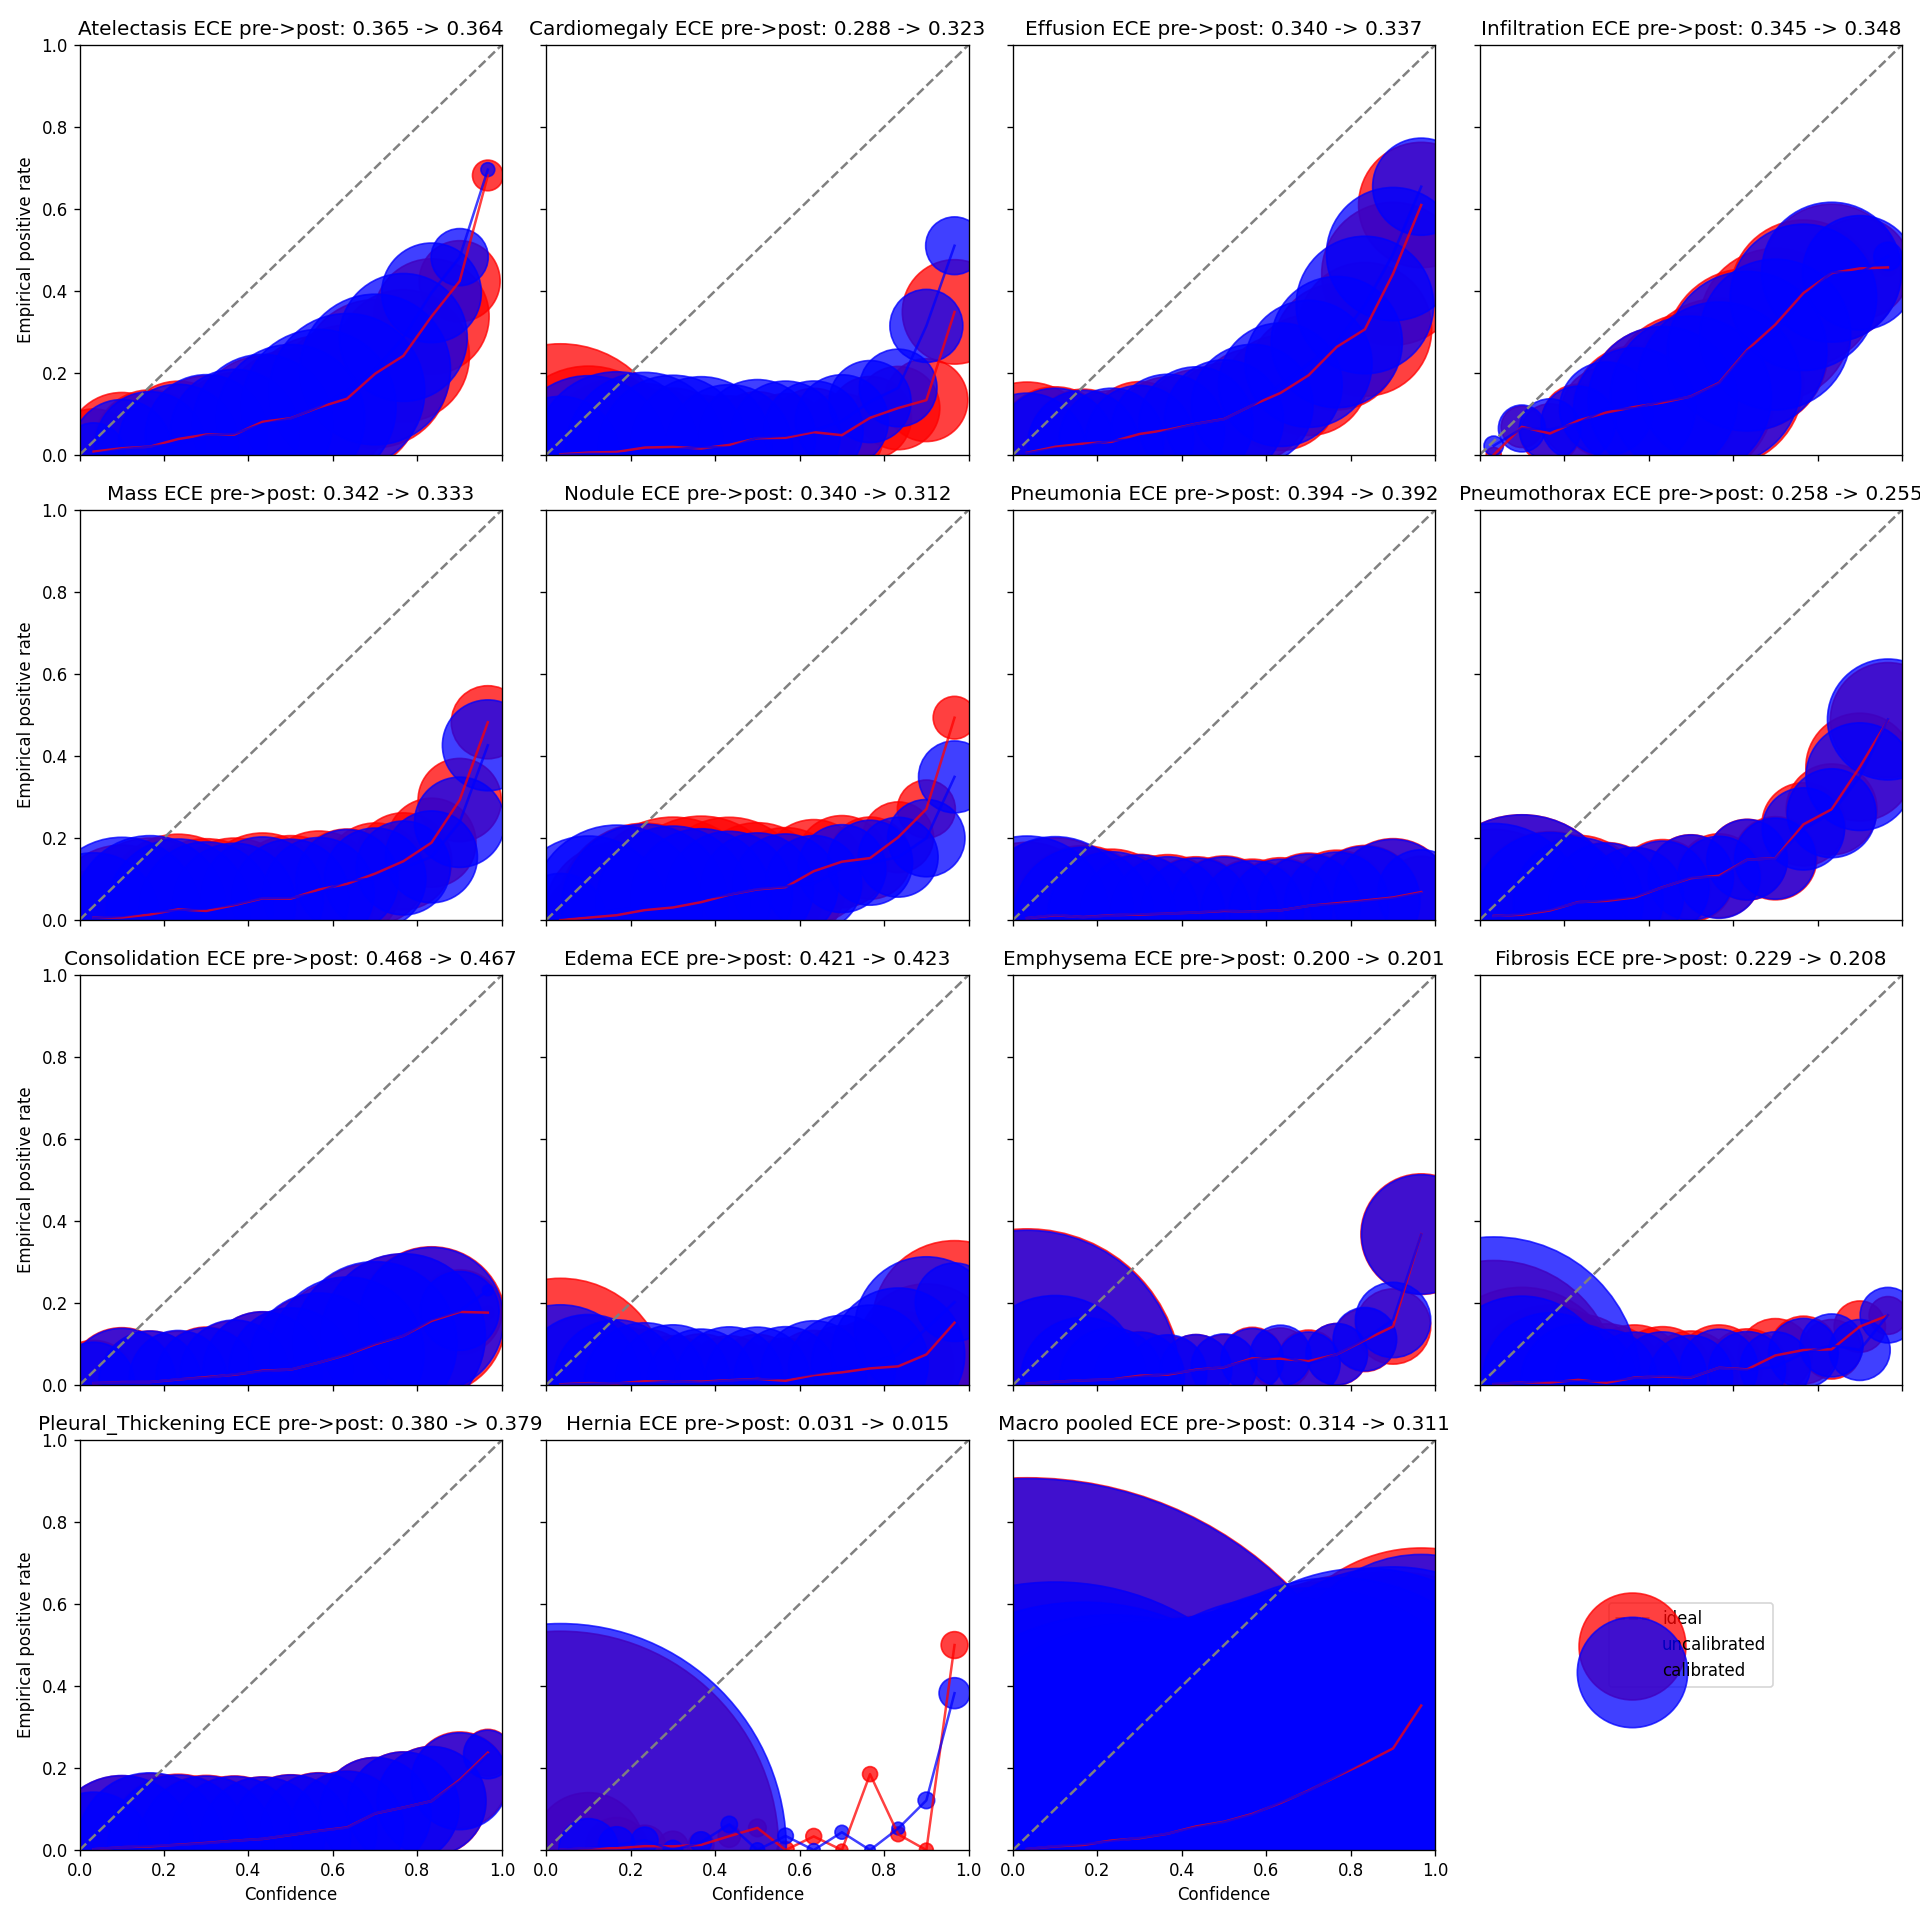
\includegraphics[width=0.8\linewidth]{../results/reliability_diagram.png}
\caption{Reliability diagram generated by \texttt{make calibrate}.}
\end{figure}
}{Calibration figure not found at compile time.}

\subsection{RSNA Overlay Figure}

\IfFileExists{../results/overlays/rsna/rsna_grid.png}{
\begin{figure}[H]
\centering
\includegraphics[width=0.95\linewidth]{../results/overlays/rsna/rsna_grid.png}
\caption{RSNA Pneumonia/Lung Opacity Grad-CAM review grid. This is a weak engineering artifact, not clinical evidence.}
\end{figure}
}{RSNA overlay grid not found at compile time.}

\subsection{CAM Threshold Sweep: Scale vs. Position Error}

The RSNA grounding numbers in the summary table above come from a single operating
point. To understand what drives the near-zero mAP@0.5 despite a pointing-game score
well above chance, \texttt{cam\_threshold} was swept over seven values on the RSNA
\textbf{validation} split (\texttt{results/sweep/}), with CAM boxes extracted per
connected component:

\begin{center}
\begin{tabular}{ccccc}
\toprule
CAM threshold & mAP@0.5 & Mean IoU & IoU $\geq$ 0.5 & Pointing-game \\
\midrule
0.30 & 0.0000 & 0.1388 & 0.0000 & 0.5138 \\
0.40 & 0.0000 & 0.1723 & 0.0000 & 0.5138 \\
0.50 & 0.0001 & 0.2138 & 0.0183 & 0.5138 \\
0.60 & 0.0004 & 0.2570 & 0.0275 & 0.5138 \\
0.70 & 0.0013 & 0.2923 & 0.0550 & 0.5138 \\
\textbf{0.80} & \textbf{0.0045} & \textbf{0.2993} & \textbf{0.1193} & 0.5138 \\
0.90 & 0.0022 & 0.1968 & 0.0550 & 0.5138 \\
\bottomrule
\end{tabular}
\end{center}

Raising the threshold from 0.60 to 0.80 increases mAP@0.5 by a factor of $10.8\times$
(0.00042 to 0.00454) and raises the fraction of boxes reaching IoU $\geq$ 0.5 from 2.8\%
to 11.9\%; the curve is unimodal and falls again at 0.90, so shrinking the box further
is not a fix. Pointing-game accuracy, by contrast, is exactly 0.5138 at every one of the
seven thresholds. This is not a coincidence: pointing-game only checks whether the CAM's
peak activation falls inside the ground-truth box, while thresholding prunes the support
around that peak without moving it. Threshold tuning can therefore correct a scale
error but not a position error, and even at the best threshold 88\% of positives still
fail the IoU $\geq$ 0.5 criterion. This scale/position split, and the resulting gap
between a loose point-based hit rate and a strict IoU-based one, is consistent with the
benchmarked divergence between saliency-metric families reported for chest X-ray
interpretation \citep{saporta2022benchmarking}.

The flatness claim above — pointing-game constant across all seven thresholds — is a
\textbf{validation-split} finding. Threshold and extraction-method selection used only
that split; \texttt{cam\_threshold = 0.80} with \texttt{box\_extraction = multi} was
then read once, as a single confirmatory point, on the held-out RSNA test split (summary
table above): mAP@0.5 0.0091, mean IoU 0.3139, IoU $\geq$ 0.5 hit rate 0.1607, and
pointing-game 0.4286. This single test point does not itself test flatness across
thresholds; only the validation sweep does that. Three of the four localization metrics
are \emph{higher} on this test read than the corresponding validation values at
threshold 0.80 (mAP@0.5 0.0045 $\to$ 0.0091; IoU $\geq$ 0.5 hit rate 0.1193 $\to$
0.1607; mean IoU 0.2993 $\to$ 0.3139); only pointing-game moved the other way (0.5138
$\to$ 0.4286). At $n = 112$ gated positive cases, a proportion near 0.5 has a standard
error of approximately $\sqrt{0.5 \times 0.5 / 112} \approx 0.047$, so the 8.5-point gap
is about $1.8$ standard errors — consistent with sampling noise on a different image
subset rather than a systematic regression. Consistent with not tuning on test,
\texttt{cam\_threshold} and \texttt{box\_extraction} were not revisited in response to
this result.

\subsection{Artifact Audit}

\begin{longtable}{p{0.29\linewidth} p{0.1\linewidth} p{0.2\linewidth} p{0.18\linewidth} p{0.15\linewidth}}
\toprule
Artifact & Exists & Source & Status & Notes \\
\midrule
\endhead
\texttt{checkpoints/baseline\_nih\_best.pt} & local & \texttt{make train} & real & epoch 4 checkpoint, git-ignored \\
\texttt{results/baseline\_nih\_eval.json} & yes & \texttt{make eval} & real & NIH metrics \\
\texttt{results/calibration\_report.json} & yes & \texttt{make calibrate} & real & ECE report \\
\texttt{results/reliability\_diagram.png} & yes & \texttt{make calibrate} & real & reliability figure \\
\texttt{results/grounding\_rsna\_eval.json} & yes & \texttt{make eval-grounding-rsna} & real & pneumonia only \\
\texttt{results/overlays/rsna/rsna\_grid.png} & yes & \texttt{make eval-grounding-rsna} & review artifact & not clinical evidence \\
\texttt{data/vqa/*.jsonl} & local & \texttt{make vqa-dataset} & generated, git-ignored & weak VQA supervision exists locally \\
\texttt{results/vlm\_zero\_shot\_eval.json} & yes & \texttt{make eval-vlm-zero-shot} & partial/blocker & rule-based baseline computed; VLM backend missing \texttt{bitsandbytes} \\
\texttt{results/vlm\_lora\_train.json} & yes & smoke/blocker check & not trained & adapter training implemented; current artifact has zero epochs \\
\bottomrule
\end{longtable}

\section{Limitations and Future Work}

The current artifacts do not support clinical use. There has been no prospective evaluation, no deployment review, and no subgroup performance audit.

NIH labels are noisy silver-standard labels. Calibration improved ECE only slightly and remains imperfect. RSNA grounding is limited to NIH \texttt{Pneumonia} evaluated against RSNA \texttt{Lung Opacity}; no other localization claim is supported.

The VQA path is rule-based and fixed-template. It is not a free-text medical chatbot. QLoRA/VLM adapter training is implemented but not trained in the current artifacts. Future work may include VQA dataset generation, zero-shot VLM evaluation, optional QLoRA training, VLM comparison, and Claude/Gemini review, but none of those should be claimed before their artifacts exist.

\appendix
\section{Appendix}

\subsection{Exact Commands}

\begin{verbatim}
make install
make lint
make test
make train
make eval
make calibrate
make prepare-rsna
make eval-grounding-rsna
\end{verbatim}

\subsection{Next Commands}

For reproduction in a fresh GPU environment:

\begin{verbatim}
git clone https://github.com/ColdVI/medguard-cxr.git
cd medguard-cxr
pip install -e ".[dev]"
make lint
make test
make train
make eval
make calibrate
make prepare-rsna
make eval-grounding-rsna
\end{verbatim}

\subsection{Release Checklist}

\begin{itemize}
  \item Real classifier checkpoint present.
  \item NIH evaluation JSON present.
  \item Calibration report and reliability diagram present.
  \item RSNA pneumonia grounding report present.
  \item README/model card/datasheet updated with real numbers only.
  \item VLM/QLoRA explicitly marked not trained.
  \item Research-only disclaimer visible.
\end{itemize}

\subsection{Do Not Claim}

Do not claim clinical validation, patient-care readiness, broad multi-abnormality localization, QLoRA training, free-text VLM behavior, or subgroup fairness from the current artifacts.


\end{document}
